% NEEDS TO BE COMPILED WITH pdflatex

\documentclass[portrait,a0paper]{baposter}

\usepackage{graphicx}
\usepackage[percent]{overpic}
\usepackage[utf8]{inputenc}
\usepackage[detect-weight]{siunitx}
\usepackage{tabto}
\usepackage{booktabs}
\usepackage{amsmath}
\usepackage{float}
\usepackage{multirow}
\usepackage[hyphens]{url}
\usepackage{enumitem}
\usepackage{ragged2e}
\usepackage{qrcode}
\usepackage{acro}
\usepackage{textcomp}

\newlength{\mytextsize}
\setlength{\unitlength}{1.0cm}

%###########################################################################################################################
% Customize here ############################################################################################################

\def\posterTitle{%
    Bottleneck identification for constraint relaxation\\
    in resource-constrained project scheduling
}
\def\posterAuthor{%
    Lukáš Nedbálek
}
\def\posterSchool{%
    Faculty of Mathematics and Physics, Charles University
}
\def\posterYear{%
    2024
}
\def\posterLogoFaculty{logos/mff-white.pdf}
\def\posterLogoSchool{logos/uk-white.pdf}

\definecolor{maincolor}{RGB}{60,80,135}
\definecolor{headercolor}{RGB}{255,255,255}
\definecolor{textbackgroundcolor}{RGB}{255,255,255}
\definecolor{highlightcolor}{RGB}{70,150,255}
\colorlet{highlightbackgroundcolorOne}{blue!60!cyan!10}
\colorlet{highlightbackgroundcolorTwo}{blue!60!cyan!10}
\def\backgroundcolor{gray!25}

% \def\headerfont{\bf\Large\sffamily}
\def\headerfont{\bf\sffamily\fontsize{13.5}{8}\selectfont}

\usepackage[scaled]{helvet}
% Uncomment for non-serif text font
% \renewcommand*\familydefault{\sfdefault}

%###########################################################################################################################
% My own macros and commands ###############################################################################################

% Custom red markings for TODO items
\newcommand{\todo}[1]{%
    \textcolor{red}{\textbf{#1}}% Bold and red text
    \PackageWarning{TODO}{#1}% Warning in LaTeX log
}
% Custom headerbox command to left-align text
\newcommand{\leftalignedheaderbox}[3]{\headerbox{\hspace{0.1em}#1}{#2}{%
    % Uncomment for left-aligned text
    % \RaggedRight{%
    #3
    % }
}}
\newcommand{\highlightheaderbox}[3]{\leftalignedheaderbox{#1}{#2,%
boxColorOne=highlightbackgroundcolorOne,boxColorTwo=highlightbackgroundcolorTwo%
}{#3}}
\newcommand{\footerbox}[2]{\headerbox{}{%
#1,%
headershape=rectangle,above=bottom,borderColor=maincolor, boxheaderheight=1pt%
}{#2}}

\newcommand{\highlight}[1]{\textbf{\color{highlightcolor}#1}}
\newcommand{\indicator}[2]{\operatorname{#1}_{#2}}
\newcommand{\indMRUR}[1]{\indicator{MRUR}{#1}}
\newcommand{\indAUAU}[1]{\indicator{AUAU}{#1}}

% first  \ac{...}
% second \ac{...}
% long   \acl{...}
% short  \acs{...}
% full   \acf{...}
% Capitalize first letter of command to capitalize acronym


\DeclareAcronym{aps}{
    short=APS,
    long=Advanced Planning and Scheduling,
}

\DeclareAcronym{rcpsp}{
    short=RCPSP,
    long=Resource-Constrained Project Scheduling Problem
}

\DeclareAcronym{ebm}{
    short=EBM,
    long=Execution Bottleneck Machine
}

% Metrics
\DeclareAcronym{mw}{
    short=MW,
    long=Machine Workload
}
\DeclareAcronym{mur}{
    short=MUR,
    long=Machine Utilization Rate
}
\DeclareAcronym{auad}{
    short=AUAD,
    long=Average Uninterrupted Active Duration
}

\DeclareAcronym{mrw}{
    short=MRW,
    long=Machine Resource Workload
}
\DeclareAcronym{mrur}{
    short=MRUR,
    long=Machine Resource Utilization Rate
}
\DeclareAcronym{auac}{
    short=AUAC,
    long=Average Uninterrupted Active Consumption
}


%###########################################################################################################################
\begin{document}
\begin{poster}
{
    grid=false,
    eyecatcher=false, % Custom main header
    columns=6, % for flexibility -- changing 2/3 columns with columnspan
    %
    background=plain,
    bgColorOne=\backgroundcolor,
    %
    headerfont={\headerfont},
    headerFontColor=headercolor,
    headershape=rectangle, %rectangle,
    headershade=plain,
    headerColorOne=maincolor,
    headerborder=open,
    %
    boxshade=shadetb,
    boxColorOne=textbackgroundcolor,
    boxColorTwo=textbackgroundcolor,
    textborder=rectangle, %rectangle,
    borderColor=maincolor,
    boxpadding=1em
}{}{
    % poster title
    \hspace*{-0.5mm}
    \begin{picture}(23.7, 3)
    \fboxsep0pt
    \put(-0.196, -0.6){\colorbox{maincolor}{\rule[96pt]{675.82pt}{0pt}}}
    \thicklines
    % minipage box for title and authors
    % Faculty logo
    \put(0.24,-0.24){\includegraphics[height=75pt]{\posterLogoFaculty}}
    \put(2.55, 2.35){
        \begin{minipage}[t][96pt]{0.75\textwidth}
        \begin{center}
        {\huge\bf\color{headercolor}\sffamily%
            \posterTitle \\[0.35cm]
        }
        {\large\color{headercolor}\sffamily%
            \posterAuthor
            \raisebox{0.1em}{$\bigm\lvert$}
            \posterSchool
            \raisebox{0.1em}{$\bigm\lvert$}
            \posterYear
            \\
        }
        \end{center} 
        \end{minipage}}
    \put(20.52,-0.24){\includegraphics[height=75pt]{\posterLogoSchool}}
    \end{picture} 
}{}{}
% ==========================================================================================================================
% ==========================================================================================================================
\leftalignedheaderbox{1. Problem statement}{name=problemStatement, column=0, row=0, span=4}{
    \begin{minipage}[0.4\textwidth]{0.56\textwidth}
        % \vspace{-0.85em}
        Scheduling large manufacturing systems is a difficult task.
        A commonly occurring problem is reducing the tardiness of a selected manufacturing order.
        \\[0.6em]
        To address this problem, we model a manufacturing system as the \acf{rcpsp},
        consisting of \emph{jobs} with associated \emph{precedences}, where jobs are executed on several \emph{resources}.
        The problem is extended with time-variable resource capacities for modeling working shifts.
        \\[0.6em]
        We use constraint programming for obtaining solutions to models of the problem.
        Resource constraints of those models are the focus of relaxations in this thesis.
    \end{minipage}
    \hfill
    \begin{minipage}{0.4\textwidth}
        \begin{center}
            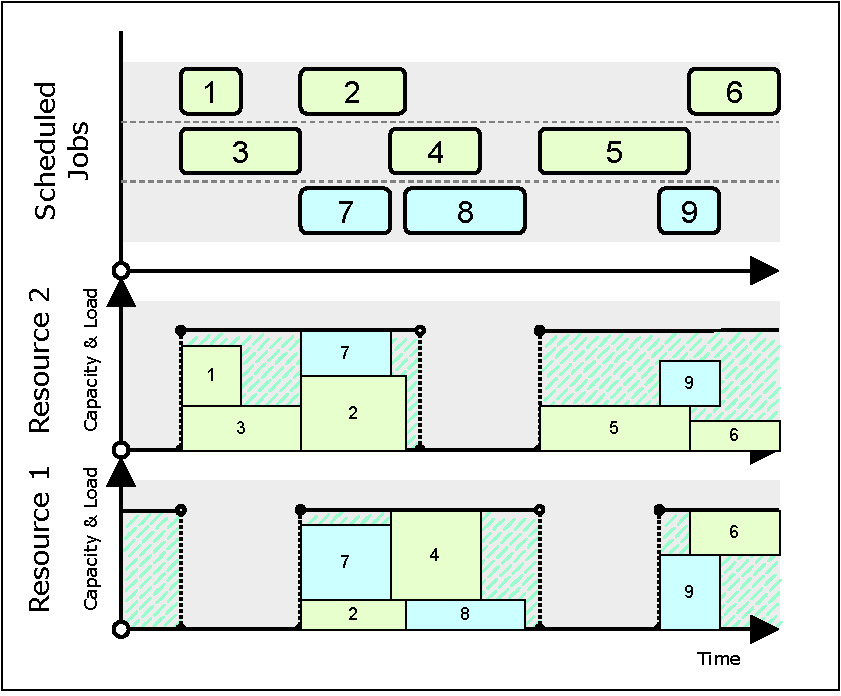
\includegraphics[width=\linewidth]{../img/Schedule.pdf}
            Example of extended RCPSP schedule
        \end{center}
    \end{minipage}
}
% --------------------------------------------------------------------------------------------------------------------------
\leftalignedheaderbox{2. Goals}{name=goals, span=2, column=4, row=0,%
bottomaligned=problemStatement
}{
    \begin{itemize}[leftmargin=*]
        \item 
            Design a method for identifying bottlenecks in obtained schedules.
        
        \item
            Propose model constraint relaxations related to the bottleneck resources in the obtained schedules.
            Such relaxations should improve the tardiness of a specific target manufacturing order
            while not modifying the original schedule much.
            Additionally, the relaxations should correspond to feasible and practical real-world implementations.
    \end{itemize}
}
% ==========================================================================================================================
\highlightheaderbox{3. Identification Indicator-based Relaxing Algorithm}{%
name=iira,column=0,span=3,below=problemStatement%
}{
    We propose two \emph{bottleneck identification indicators} for the extended \acs{rcpsp}
    --- \acf{mrur} and \acf{auau}. Each computes a single numeric value for a given resource $k$.
    \vspace{-0.5em}
    \begin{align*}
        &\indMRUR{k} = \frac{\text{total consumption of $k$ by all jobs}}%
                           {\text{total capacity of $k$ over project makespan}}
        \\
        &\indAUAU{k} = \text{average utilization over uninterrupted active periods}\\[-2.2em]
        % \\
        % &\text{where utilization during active period} = \frac{\text{total active period consumption }}{\text{total active period capacity}}.
    \end{align*}
    % The \acf{iira} identifies a bottleneck resource using an identification indicator,
    % calculates a granular resource load functions for the bottleneck resource,
    % and determines the improvement potential of granular periods through convolution.
    % It the relaxes resource capacities of the bottleneck resource
    % during the granular period with highest computed improvement potential.
    % Finally, a solution to the modified problem is found
    % and proposed capacity changes are reduced to only include utilized changes.
    The \acf{iira} works as follows:
    \begin{center}
    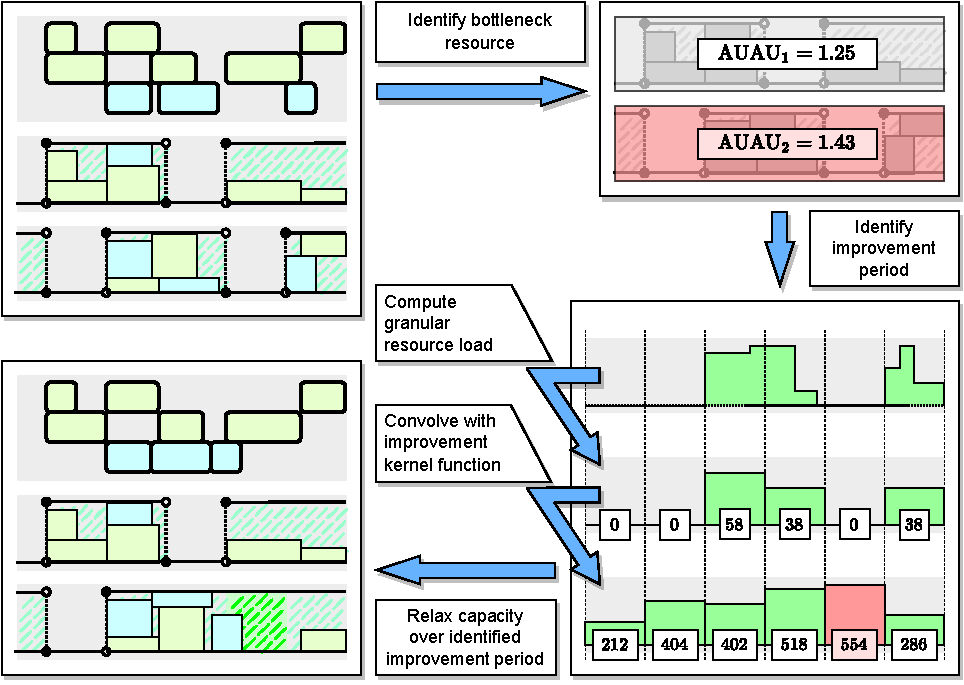
\includegraphics[width=\textwidth]{img/iira.pdf}
    \end{center}
    \vspace{-0.6em}
    The proposed resource capacity functions are reduced to only include utilized changes.
    The changes are then divided into \emph{migrations} and \emph{additions} based on available capacities
    on remaining resources.
}
% --------------------------------------------------------------------------------------------------------------------------
\highlightheaderbox{4. Schedule Suffix Interval Relaxing Algorithm}{%
name=ssira,column=3,span=3,below=problemStatement%
}{
    The \acf{ssira} relaxes \emph{suffixes of schedules} to obtain heuristic interval relaxation proposals.
    The algorithm focuses on the target manufacturing order
    by identifying improvement intervals only within its left-shift closure.
    The \emph{left-shift closure} of a manufacturing order is the set of jobs that,
    corresponding to various definitions, prevent the order from finishing earlier.
    \begin{center}
    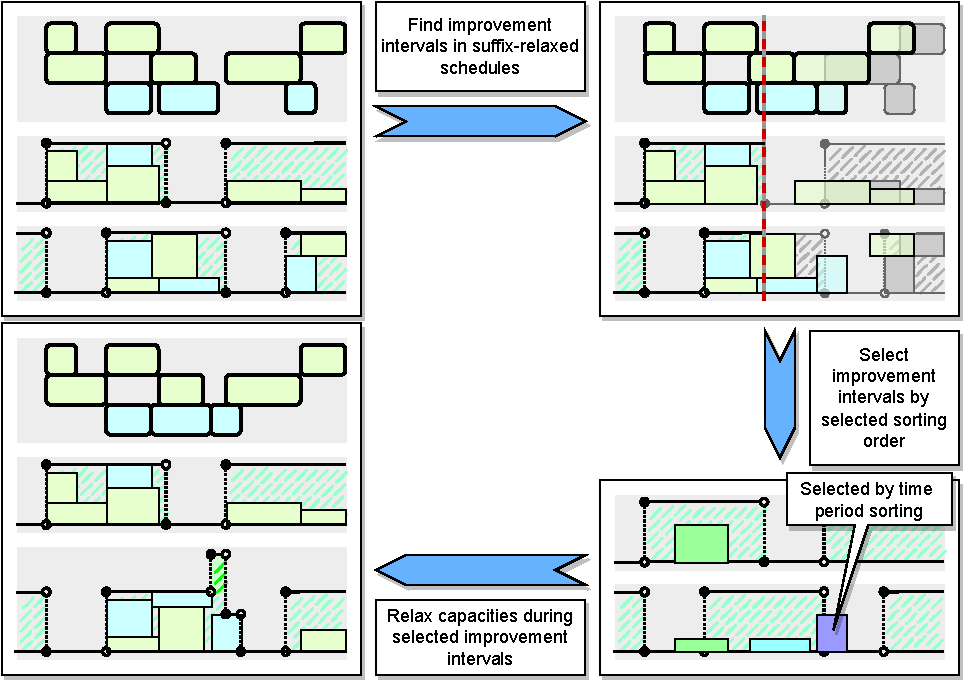
\includegraphics[width=\textwidth]{img/ssira.pdf}
    \end{center}
    \vspace{-0.6em}
    Same as in the \acs{iira}, the capacity changes are reduced and corresponding capacity \emph{migrations} and \emph{additions} are identified.
}
% ==========================================================================================================================
\leftalignedheaderbox{5. Experiments}{%
name=experiments,column=0,row=0,span=3,below=iira%
}{
    Numerical experiments were conducted to analyze the capabilities
    of the proposed methods. For that purpose, we designed a set of problem instances
    (based on PSPLIB instances) modeling the used extension of the RCPSP.

    We observed that the \highlight{SSIRA is more consistent in finding improving solutions} than the IIRA,
    while the \highlight{IIRA is able to find great improvements with low modification costs} on instances,
    where the SSIRA finds the same improvements with greater costs.
}		
% --------------------------------------------------------------------------------------------------------------------------
\leftalignedheaderbox{6. Summary}{%
name=summary,column=3,span=3,below=ssira,bottomaligned=experiments%
}{
    In this thesis, we
    \begin{itemize}[leftmargin=*]
        \item
            \highlight{designed the \acs{iira}} as a baseline solution adapting existing bottleneck identification approaches
            from the scheduling literature and proposing relaxations based on those identifications,\\[-1.8em]
        \item
            \highlight{designed the \acs{ssira}} as a novel approach to identifying schedule bottlenecks
            and relaxing related constraints in the \acs{rcpsp}, and\\[-1.8em]
        \item
            \highlight{conducted numerical experiments} showing that the \acs{iira} achieves great improvements for small costs,
            while the \acs{ssira} is more reliable in achieving improvements across various problem instances.
    \end{itemize}

    Future work could focus on modeling the relaxations as an optimization problem to obtain exact proposals
    capturing all model dependencies.
}
% Footer ===================================================================================================================
\footerbox{%
name=repository,column=2,span=4,above=bottom%
}{
    \begin{minipage}{.17\textwidth}
        \begin{center}
            % \vspace{-0.22cm}%
            \qrcode[height=2cm]{https://github.com/Krtiiik/RCPSPSandbox}%
        \end{center}
    \end{minipage}%
    \begin{minipage}{.66\textwidth}
        \textbf{\large\sffamily\color{maincolor}Project repository}
        \\[0.25em]
        \scriptsize\url{https://github.com/Krtiiik/RCPSPSandbox}
        % \vfill\hrule\vfill
        \vspace{0.55em}\hrule\vspace{0.55em}
        \hfill\textbf{\large\sffamily\color{maincolor}Bachelor thesis}
        \\[0.25em]
        \scriptsize\url{https://github.com/Krtiiik/Bottleneck-identification-for-constraint-relaxation-in-resource-constrained-project-scheduling/blob/main/thesis.pdf}
    \end{minipage}%
    \begin{minipage}{.17\textwidth}
        \begin{center}
            % \vspace{-0.22cm}%
            \qrcode[height=2cm]{https://github.com/Krtiiik/Bottleneck-identification-for-constraint-relaxation-in-resource-constrained-project-scheduling/blob/main/thesis.pdf}%
        \end{center}
    \end{minipage}%
}
\footerbox{%
name=supervisor,column=0,span=2,above=bottom,aligned=repository%
}{
    \textbf{\sffamily\large\color{maincolor}Supervisor}
    \\[0.4em]
    {\large RNDr. Jiří Švancara, Ph.D.}
    \\[0.1em]
    Department of Theoretical Computer Science and Mathematical Logic, MFF UK
}
\end{poster}
\end{document}
